\documentclass[12pt]{article}
\usepackage[margin=1.5cm]{geometry}
\usepackage{pdflscape}
\usepackage{graphicx}
\usepackage{caption}
\usepackage{tikz}
\usetikzlibrary{shapes.geometric, arrows.meta, positioning, fit, backgrounds}
\tikzset{
  block/.style = {rectangle, rounded corners, draw=black, thick, align=center, minimum height=1.0cm, minimum width=3.4cm, fill=blue!5},
  process/.style = {rectangle, draw=black, thick, align=center, minimum height=1.0cm, minimum width=3.8cm, fill=green!6},
  decision/.style = {diamond, aspect=2, draw=black, thick, align=center, inner sep=1pt, fill=orange!8},
  io/.style = {trapezium, trapezium left angle=70, trapezium right angle=110, draw=black, thick, align=center, minimum height=1.0cm, minimum width=3.4cm, fill=purple!6},
  line/.style = {-{Latex[length=3mm]}, thick},
  groupbox/.style = {draw=black!60, dashed, rounded corners, inner sep=6pt}
}
\begin{document}
\begin{landscape}
\begin{center}
\resizebox{0.94\linewidth}{!}{%
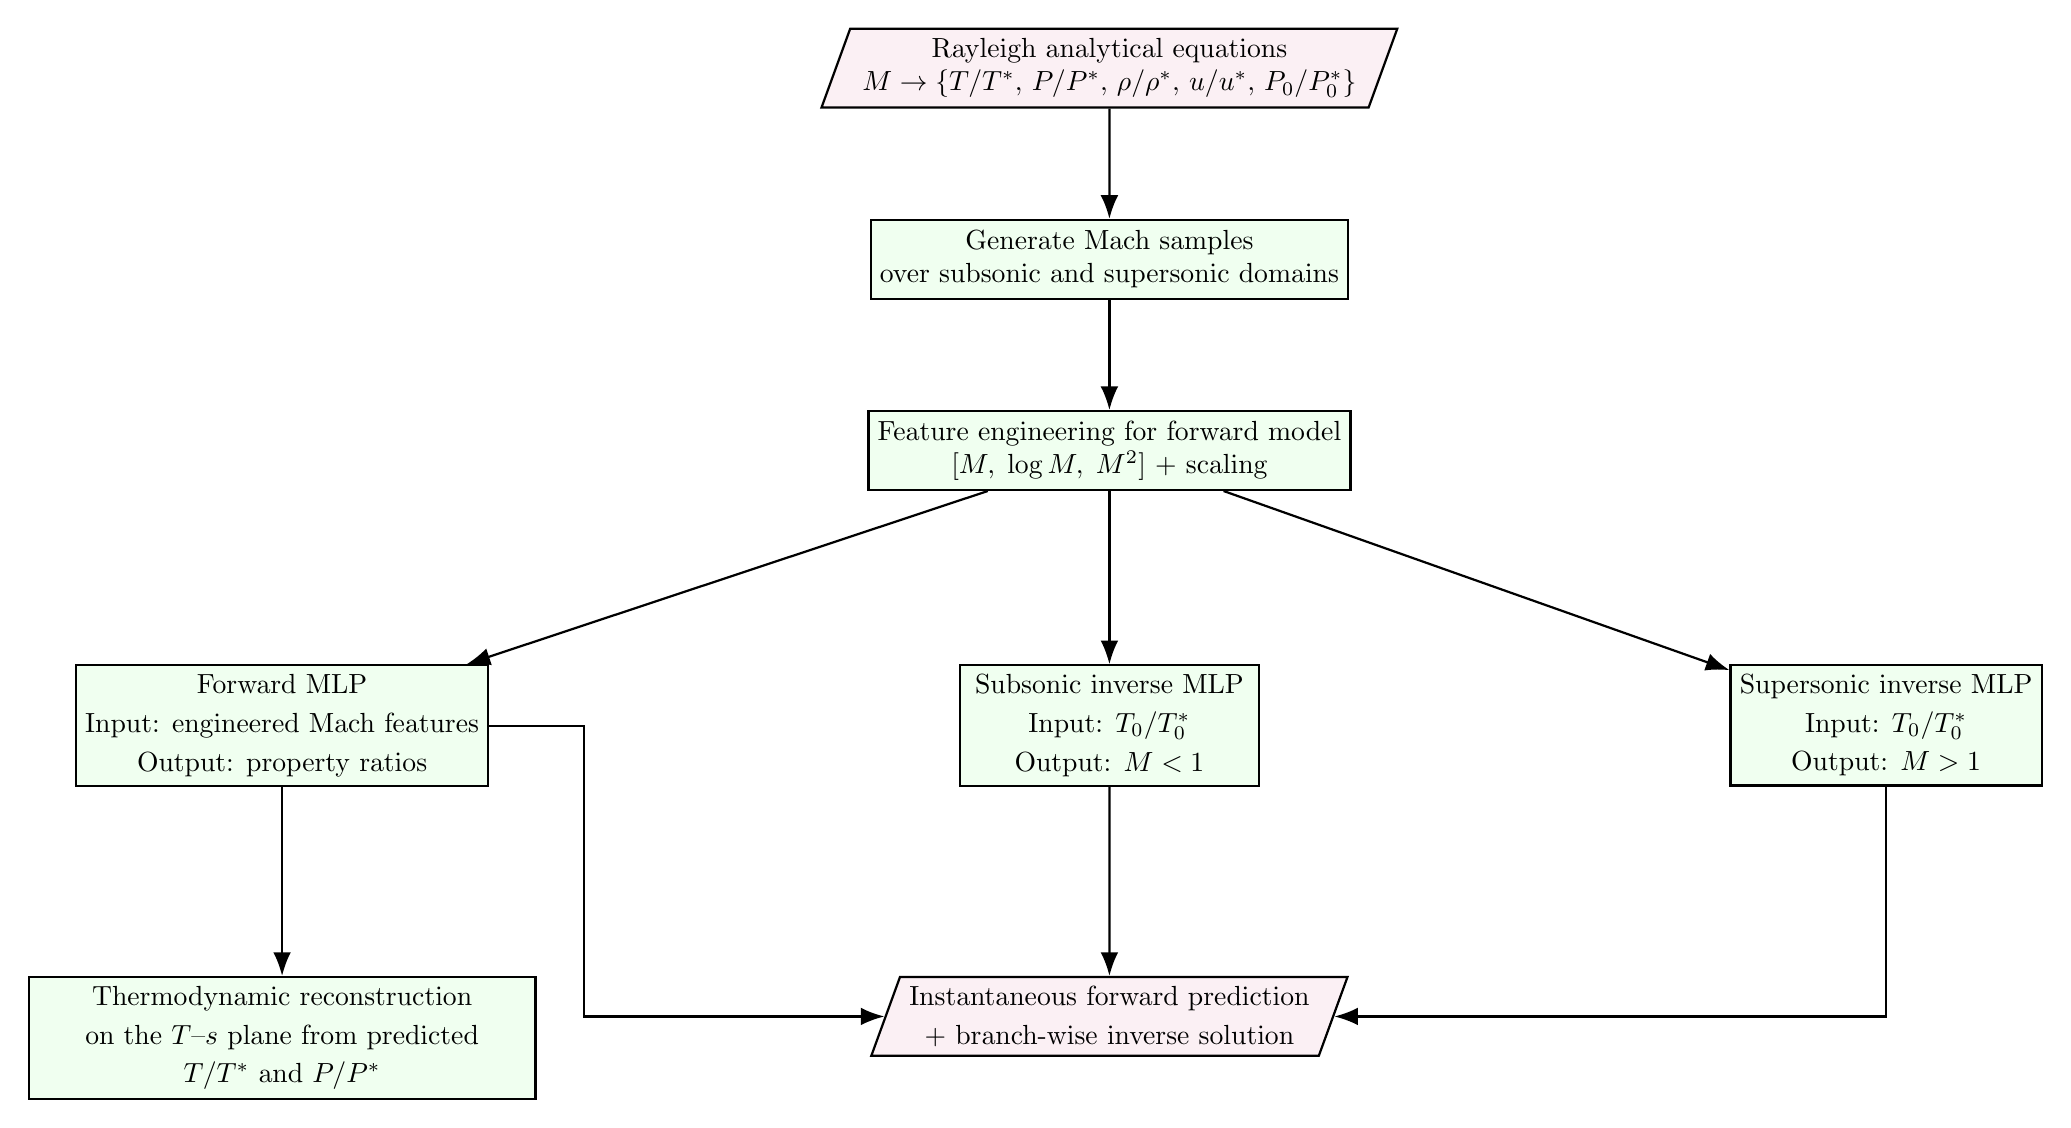
\begin{tikzpicture}[node distance=1.4cm and 2.0cm]

% Top chain
\node[io] (eq) {Rayleigh analytical equations\\ $M \rightarrow \{T/T^*,\,P/P^*,\,\rho/\rho^*,\,u/u^*,\,P_0/P_0^*\}$};

\node[process, below=of eq] (gen) {Generate Mach samples\\ over subsonic and supersonic domains};

\node[process, below=of gen] (feat) {Feature engineering for forward model\\ $[M,\;\log M,\;M^2]$ + scaling};

% Main model row
\node[process, below left=2.2cm and 4.8cm of feat] (fwd) {Forward MLP\\[2pt]
Input: engineered Mach features\\[2pt]
Output: property ratios};

\node[process, below=2.2cm of feat] (sub) {Subsonic inverse MLP\\[2pt]
Input: $T_0/T_0^*$\\[2pt]
Output: $M<1$};

\node[process, below right=2.2cm and 4.8cm of feat] (sup) {Supersonic inverse MLP\\[2pt]
Input: $T_0/T_0^*$\\[2pt]
Output: $M>1$};

% Bottom row
\node[process, below=2.4cm of fwd, text width=6.2cm] (ts) {Thermodynamic reconstruction\\[2pt]
on the $T$--$s$ plane from predicted\\[2pt]
$T/T^*$ and $P/P^*$};

\node[io, below=2.4cm of sub] (pred) {Instantaneous forward prediction\\[2pt]
+ branch-wise inverse solution};

% Connections
\draw[line] (eq) -- (gen);
\draw[line] (gen) -- (feat);

\draw[line] (feat) -- (fwd);
\draw[line] (feat) -- (sub);
\draw[line] (feat) -- (sup);

\draw[line] (fwd.south) -- (ts.north);
\draw[line] (fwd.east) -- ++(12mm,0) |- (pred.west);
\draw[line] (sub) -- (pred);
\draw[line] (sup) |- (pred);

\end{tikzpicture}%
}
\captionof{figure}{Rayleigh-flow surrogate architecture. The forward model learns the mapping from Mach number to thermodynamic property ratios using engineered Mach-based features, while the inverse problem is resolved through separate subsonic and supersonic expert networks. The forward predictions are additionally used for thermodynamic reconstruction on the $T$--$s$ plane.}
\label{fig:rayleigh_flowchart}
\end{center}
\end{landscape}

\begin{landscape}
\begin{center}
\resizebox{0.92\linewidth}{!}{%
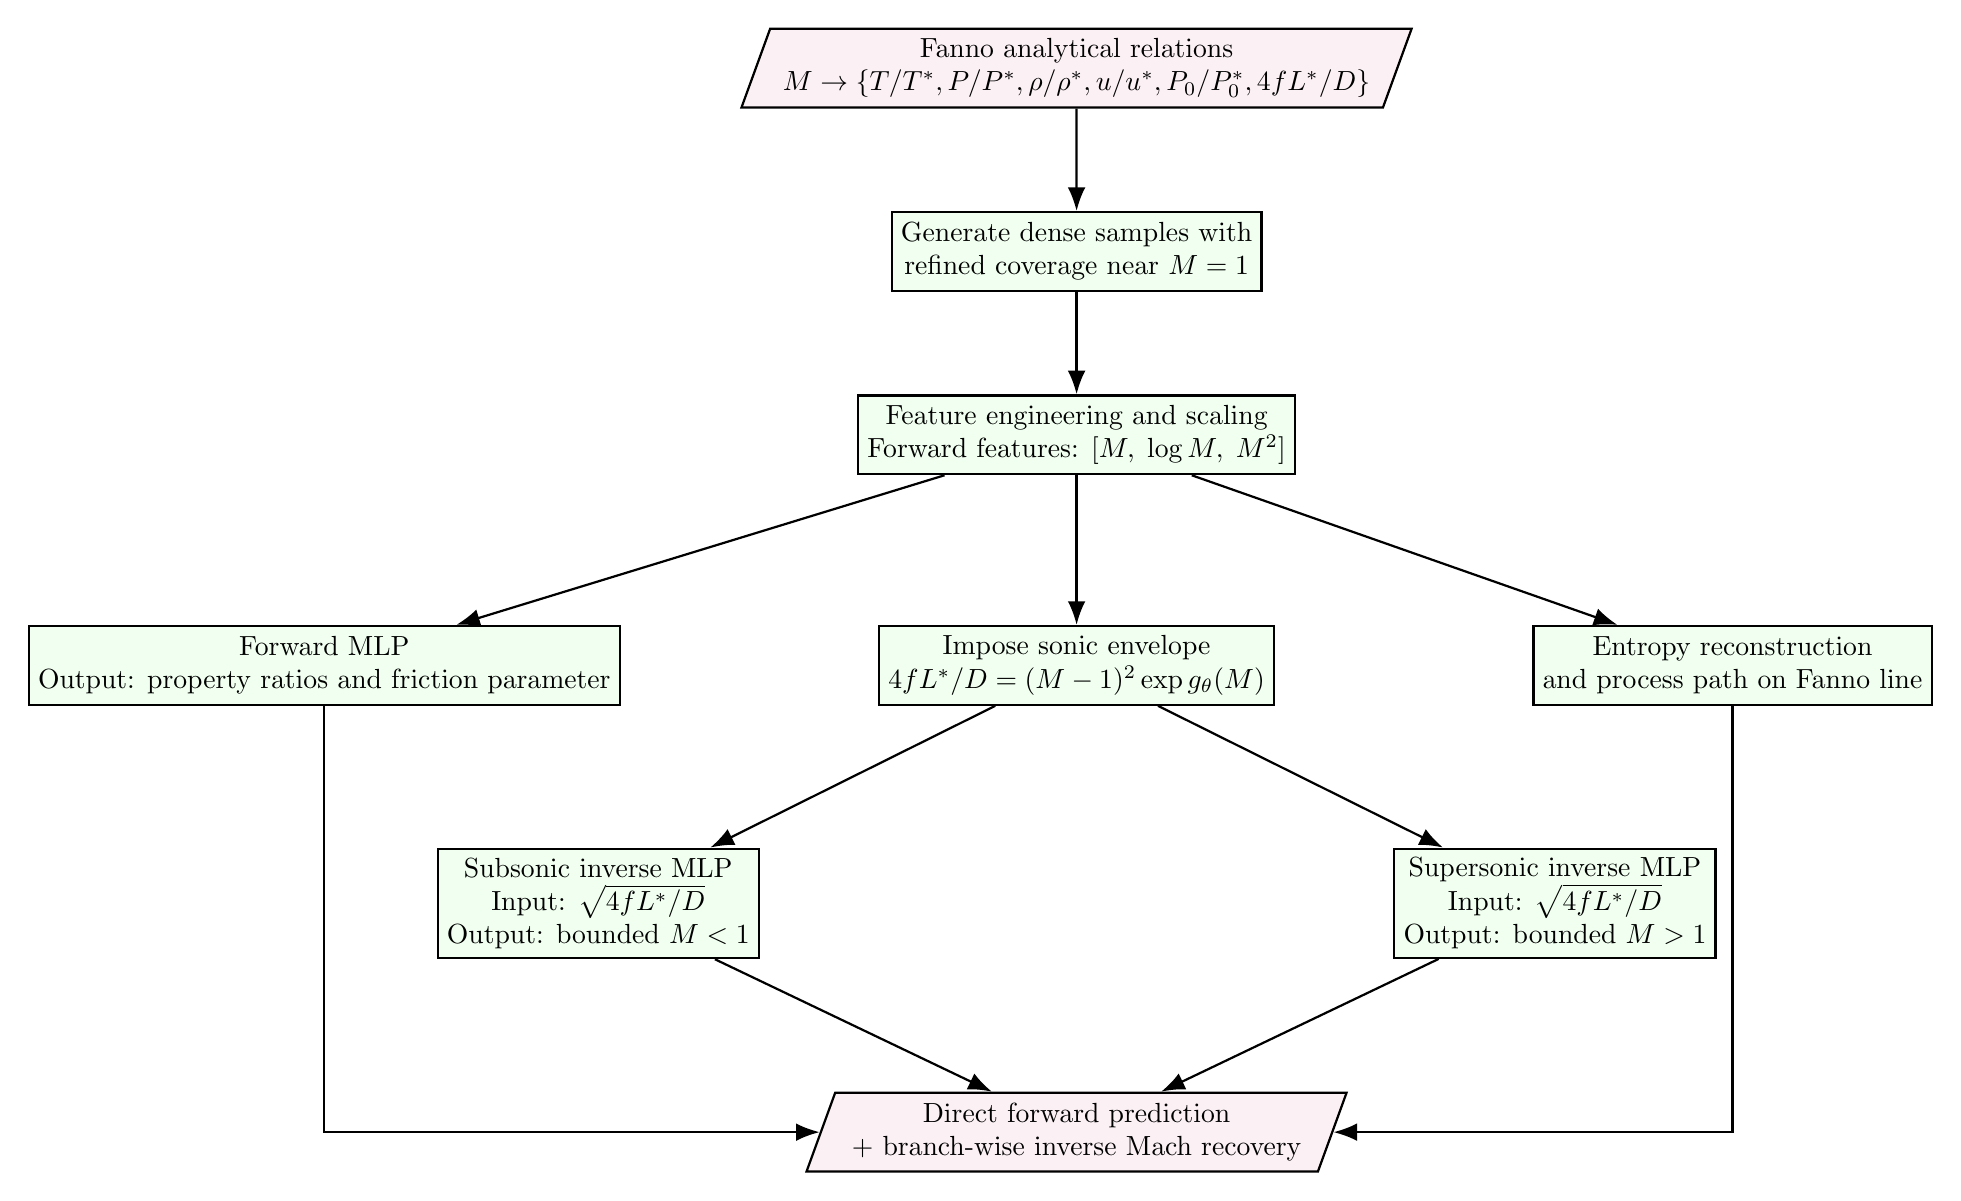
\begin{tikzpicture}[node distance=1.3cm and 1.8cm]
\node[io] (eq) {Fanno analytical relations\\ $M \rightarrow \{T/T^*,P/P^*,\rho/\rho^*,u/u^*,P_0/P_0^*,4fL^*/D\}$};
\node[process, below=of eq] (gen) {Generate dense samples with\\ refined coverage near $M=1$};
\node[process, below=of gen] (feat) {Feature engineering and scaling\\ Forward features: $[M,\;\log M,\;M^2]$};

\node[process, below left=1.9cm and 3.0cm of feat] (fwd) {Forward MLP\\ Output: property ratios and friction parameter};
\node[process, below=1.9cm of feat] (logt) {Impose sonic envelope\\ $4fL^*/D=(M-1)^2\exp g_\theta(M)$};
\node[process, below right=1.9cm and 3.0cm of feat] (ts) {Entropy reconstruction\\ and process path on Fanno line};

\node[process, below left=1.8cm and 1.5cm of logt] (sub) {Subsonic inverse MLP\\ Input: $\sqrt{4fL^*/D}$\\ Output: bounded $M<1$};
\node[process, below right=1.8cm and 1.5cm of logt] (sup) {Supersonic inverse MLP\\ Input: $\sqrt{4fL^*/D}$\\ Output: bounded $M>1$};

\node[io, below=4.9cm of logt] (out) {Direct forward prediction\\ + branch-wise inverse Mach recovery};

\draw[line] (eq) -- (gen);
\draw[line] (gen) -- (feat);
\draw[line] (feat) -- (fwd);
\draw[line] (feat) -- (logt);
\draw[line] (feat) -- (ts);
\draw[line] (logt) -- (sub);
\draw[line] (logt) -- (sup);
\draw[line] (fwd) |- (out);
\draw[line] (sub) -- (out);
\draw[line] (sup) -- (out);
\draw[line] (ts) |- (out);
\end{tikzpicture}%
}
\captionof{figure}{Fanno-flow surrogate architecture. The forward network learns positive thermodynamic ratios and the residual function inside an exact quadratic sonic envelope. The inverse uses the regularized coordinate $\sqrt{4fL^*/D}$ and separate bounded subsonic and supersonic expert networks.}
\label{fig:fanno_flowchart}
\end{center}
\end{landscape}

\begin{landscape}
\begin{center}
\resizebox{0.92\linewidth}{!}{%
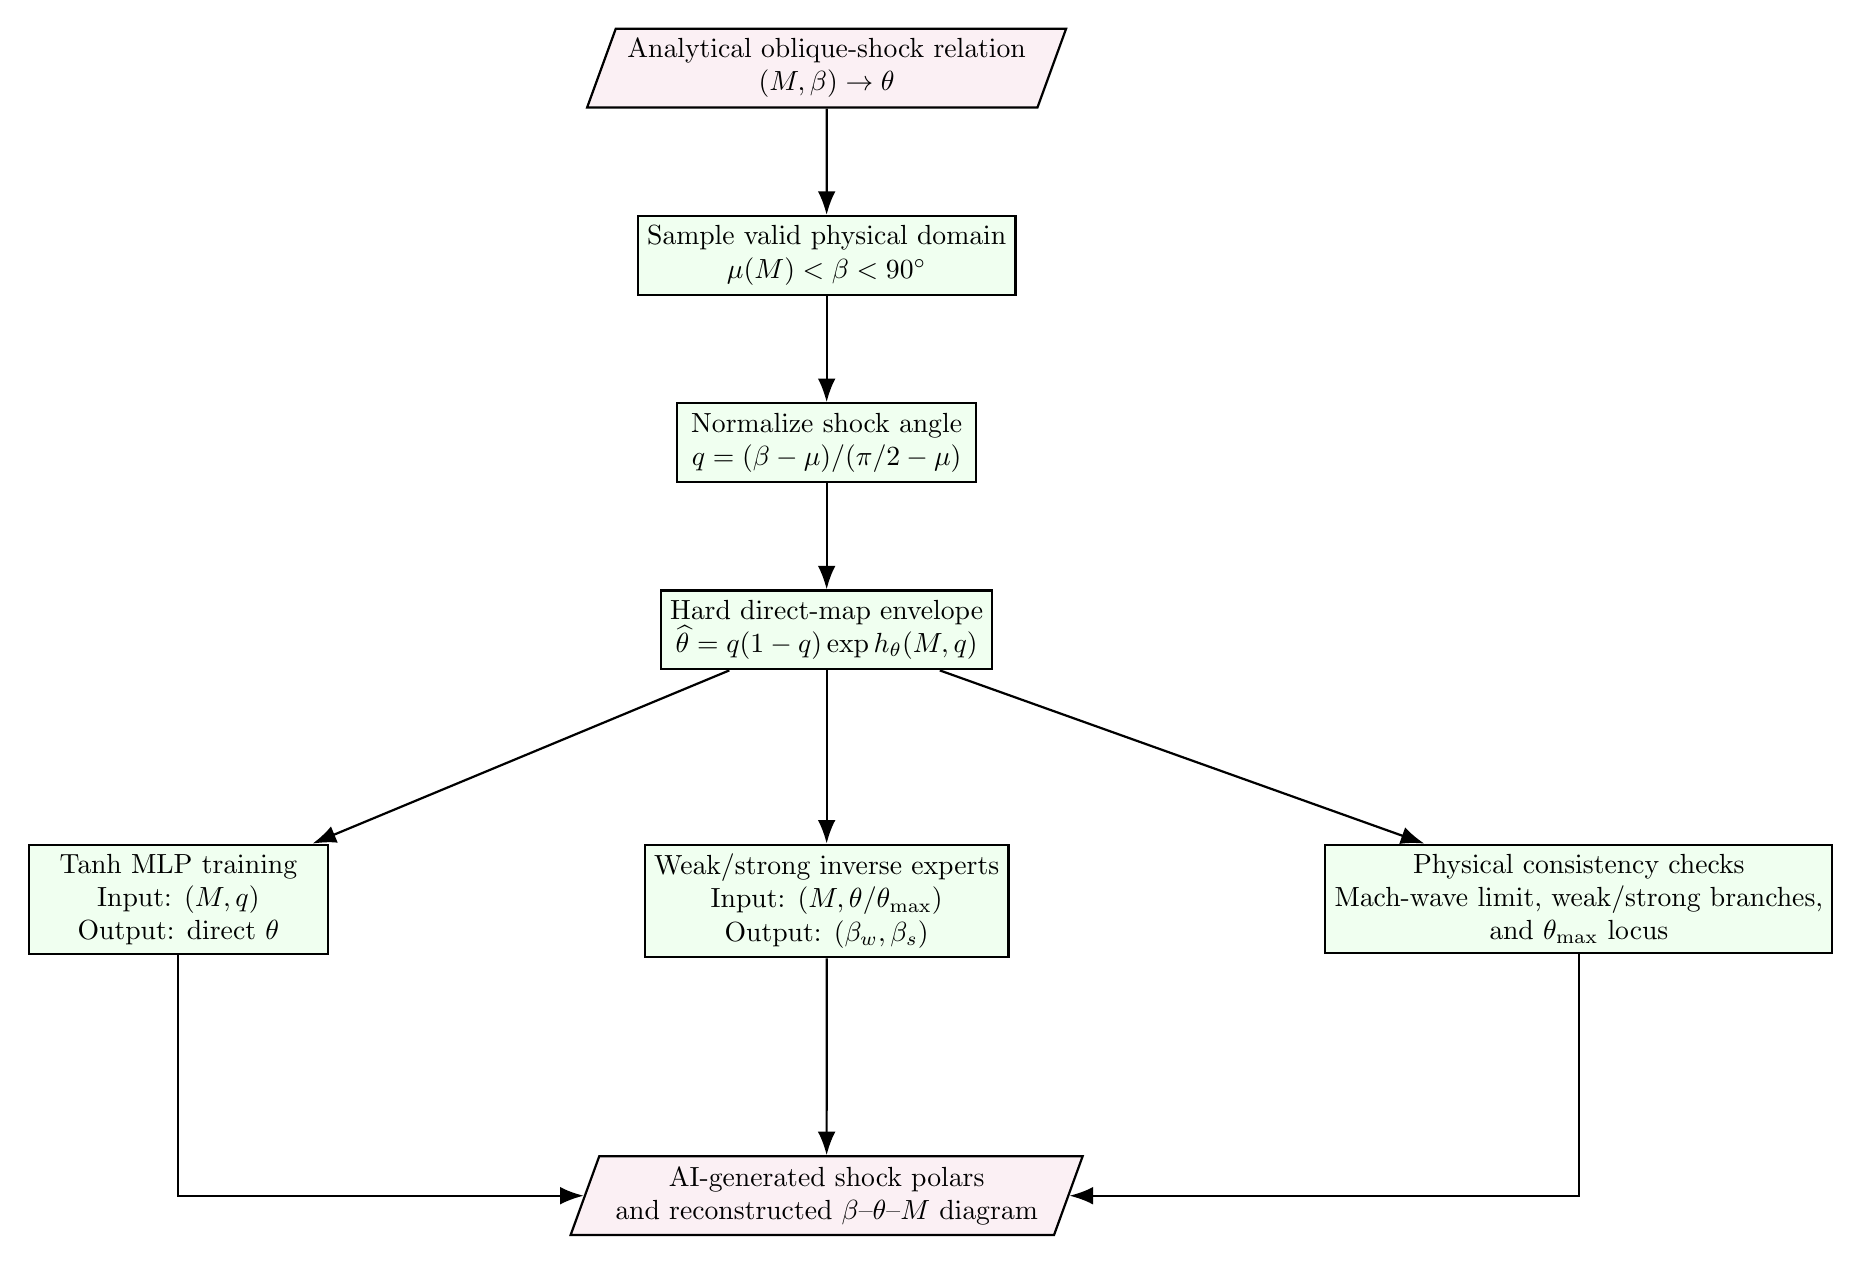
\begin{tikzpicture}[node distance=1.35cm and 1.8cm]

% Top chain
\node[io] (eq) {Analytical oblique-shock relation\\ $(M,\beta)\rightarrow \theta$};

\node[process, below=of eq] (sample) {Sample valid physical domain\\ $\mu(M)<\beta<90^\circ$};

\node[process, below=of sample] (anchor) {Normalize shock angle\\ $q=(\beta-\mu)/(\pi/2-\mu)$};

\node[process, below=of anchor] (feat) {Hard direct-map envelope\\ $\widehat\theta=q(1-q)\exp h_\theta(M,q)$};

% Middle row
\node[process, below left=2.2cm and 4.2cm of feat] (train) {Tanh MLP training\\ Input: $(M,q)$\\ Output: direct $\theta$};

\node[process, below=2.2cm of feat] (recon) {Weak/strong inverse experts\\ Input: $(M,\theta/\theta_{\max})$\\ Output: $(\beta_w,\beta_s)$};

\node[process, below right=2.2cm and 4.2cm of feat] (check) {Physical consistency checks\\ Mach-wave limit, weak/strong branches,\\ and $\theta_{\max}$ locus};

% Bottom output
\node[io, below=2.5cm of recon] (out) {AI-generated shock polars\\ and reconstructed $\beta$--$\theta$--$M$ diagram};

% Arrows
\draw[line] (eq) -- (sample);
\draw[line] (sample) -- (anchor);
\draw[line] (anchor) -- (feat);

\draw[line] (feat) -- (train);
\draw[line] (feat) -- (recon);
\draw[line] (feat) -- (check);

\draw[line] (train) |- (out);
\draw[line] (recon) -- (out);
\draw[line] (check) |- (out);

\end{tikzpicture}%
}
\captionof{figure}{Oblique-shock surrogate workflow. The direct map uses an exact endpoint envelope, while separate bounded inverse outputs represent the weak and strong branches.}
\label{fig:oblique_flowchart}
\end{center}
\end{landscape}

\begin{landscape}
\begin{center}
\resizebox{0.90\linewidth}{!}{%
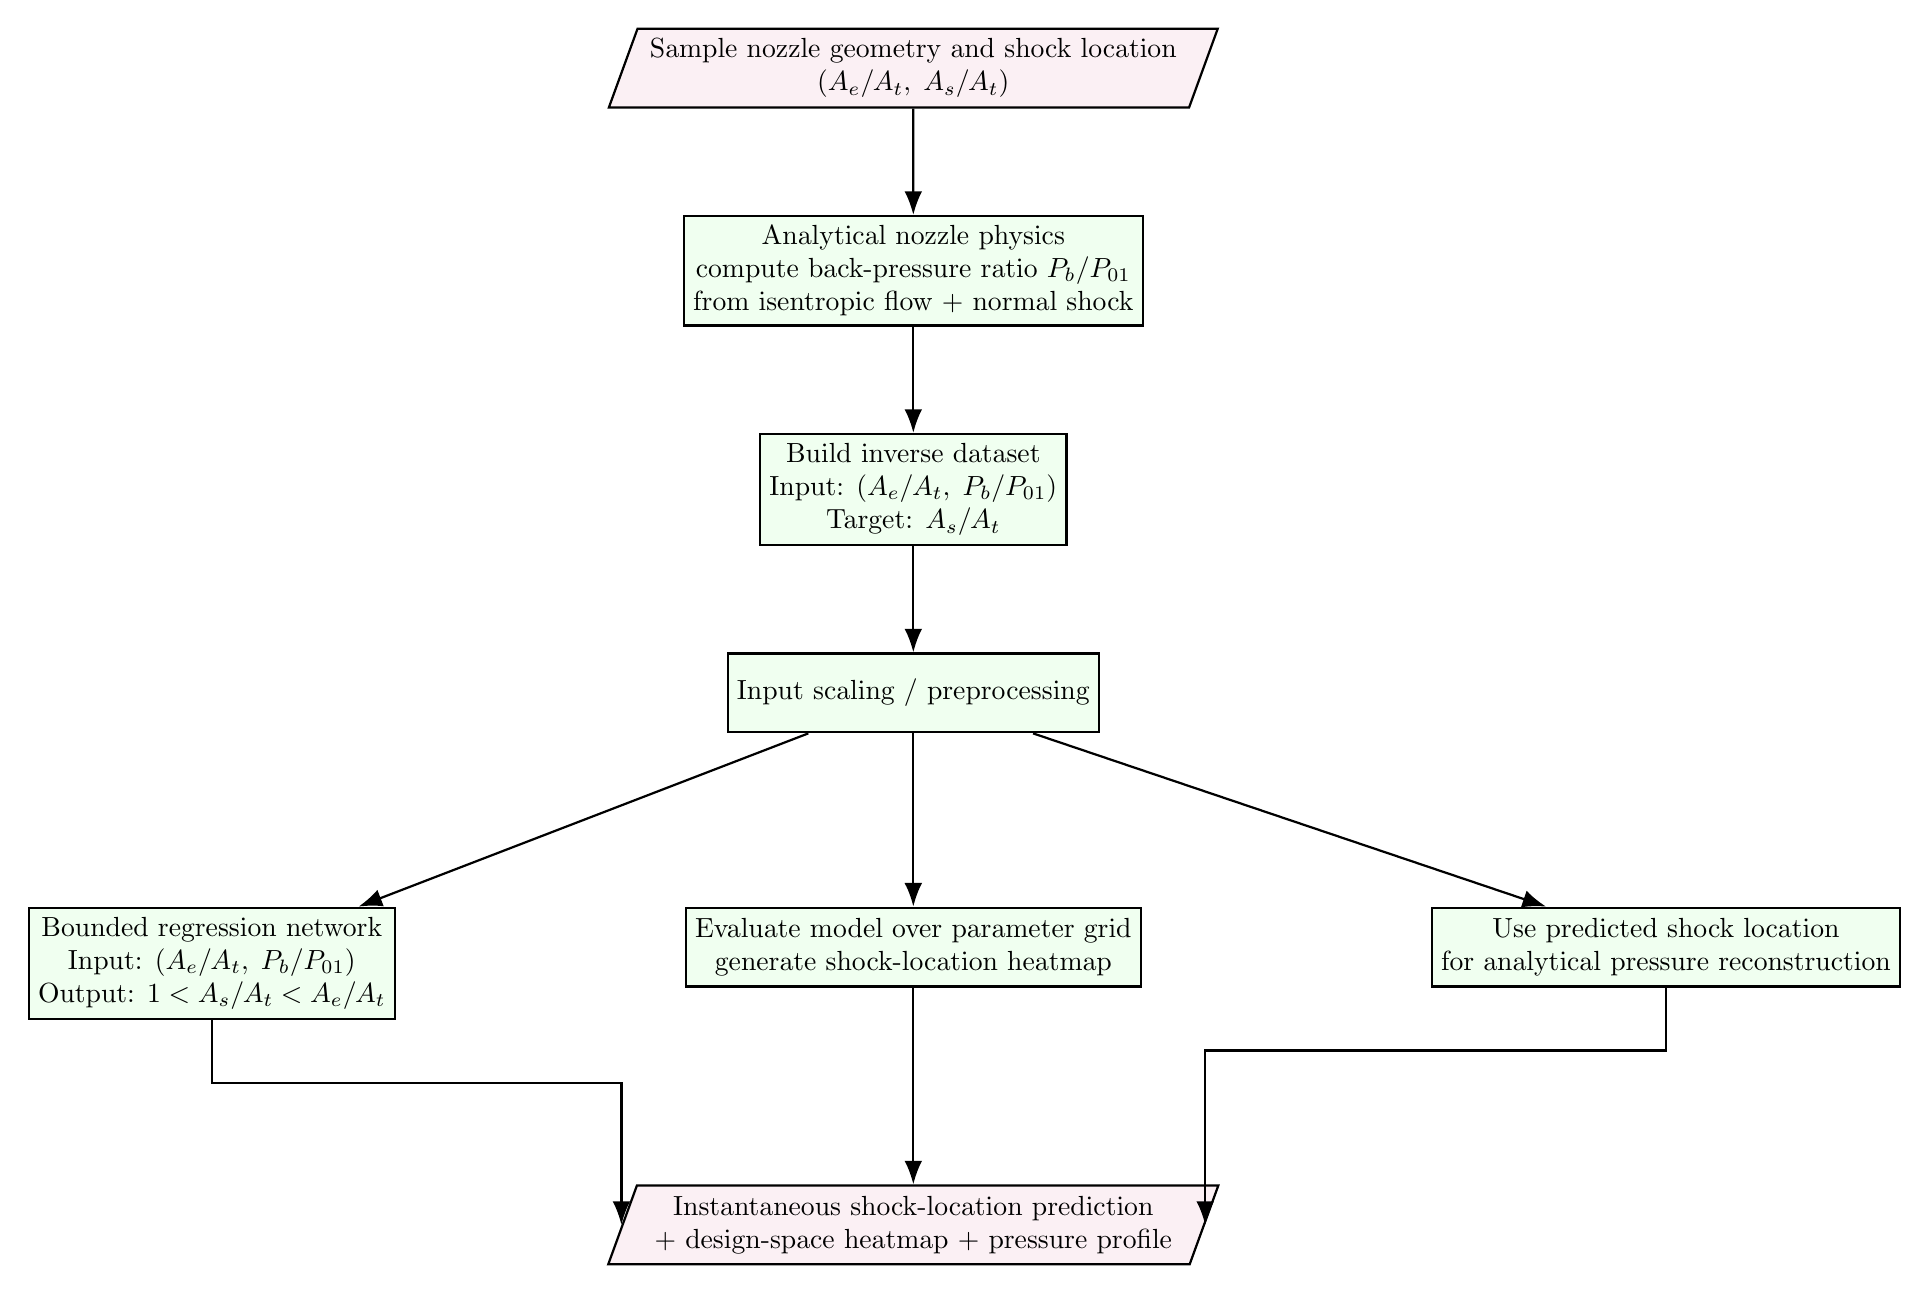
\begin{tikzpicture}[node distance=1.35cm and 1.8cm]

% Top chain
\node[io] (sample) {Sample nozzle geometry and shock location\\ $(A_e/A_t,\;A_s/A_t)$};

\node[process, below=of sample] (physics) {Analytical nozzle physics\\ compute back-pressure ratio $P_b/P_{01}$\\ from isentropic flow + normal shock};

\node[process, below=of physics] (dataset) {Build inverse dataset\\ Input: $(A_e/A_t,\;P_b/P_{01})$\\ Target: $A_s/A_t$};

\node[process, below=of dataset] (scale) {Input scaling / preprocessing};

% Middle row
\node[process, below left=2.2cm and 4.2cm of scale] (train) {Bounded regression network\\ Input: $(A_e/A_t,\;P_b/P_{01})$\\ Output: $1<A_s/A_t<A_e/A_t$};

\node[process, below=2.2cm of scale] (heatmap) {Evaluate model over parameter grid\\ generate shock-location heatmap};

\node[process, below right=2.2cm and 4.2cm of scale] (recon) {Use predicted shock location\\ for analytical pressure reconstruction};

% Bottom output
\node[io, below=2.5cm of heatmap] (out) {Instantaneous shock-location prediction\\ + design-space heatmap + pressure profile};

% Arrows
\draw[line] (sample) -- (physics);
\draw[line] (physics) -- (dataset);
\draw[line] (dataset) -- (scale);

\draw[line] (scale) -- (train);
\draw[line] (scale) -- (heatmap);
\draw[line] (scale) -- (recon);

\draw[line] (train.south) -- ++(0,-8mm) -| (out.west);
\draw[line] (heatmap.south) -- (out.north);
\draw[line] (recon.south) -- ++(0,-8mm) -| (out.east);

\end{tikzpicture}%
}
\captionof{figure}{Workflow of the neural-network surrogate for normal-shock location in a convergent-divergent nozzle. Synthetic inverse-design data are generated analytically by sampling nozzle geometries and shock locations, then computing the corresponding back-pressure ratio. A regression network is trained to predict the shock location directly from nozzle geometry and back pressure, and the trained model is subsequently used for real-time design-space heatmaps and analytical pressure-profile reconstruction.}
\label{fig:nozzle_flowchart}
\end{center}
\end{landscape}

\begin{landscape}
\begin{center}
\resizebox{0.92\linewidth}{!}{%
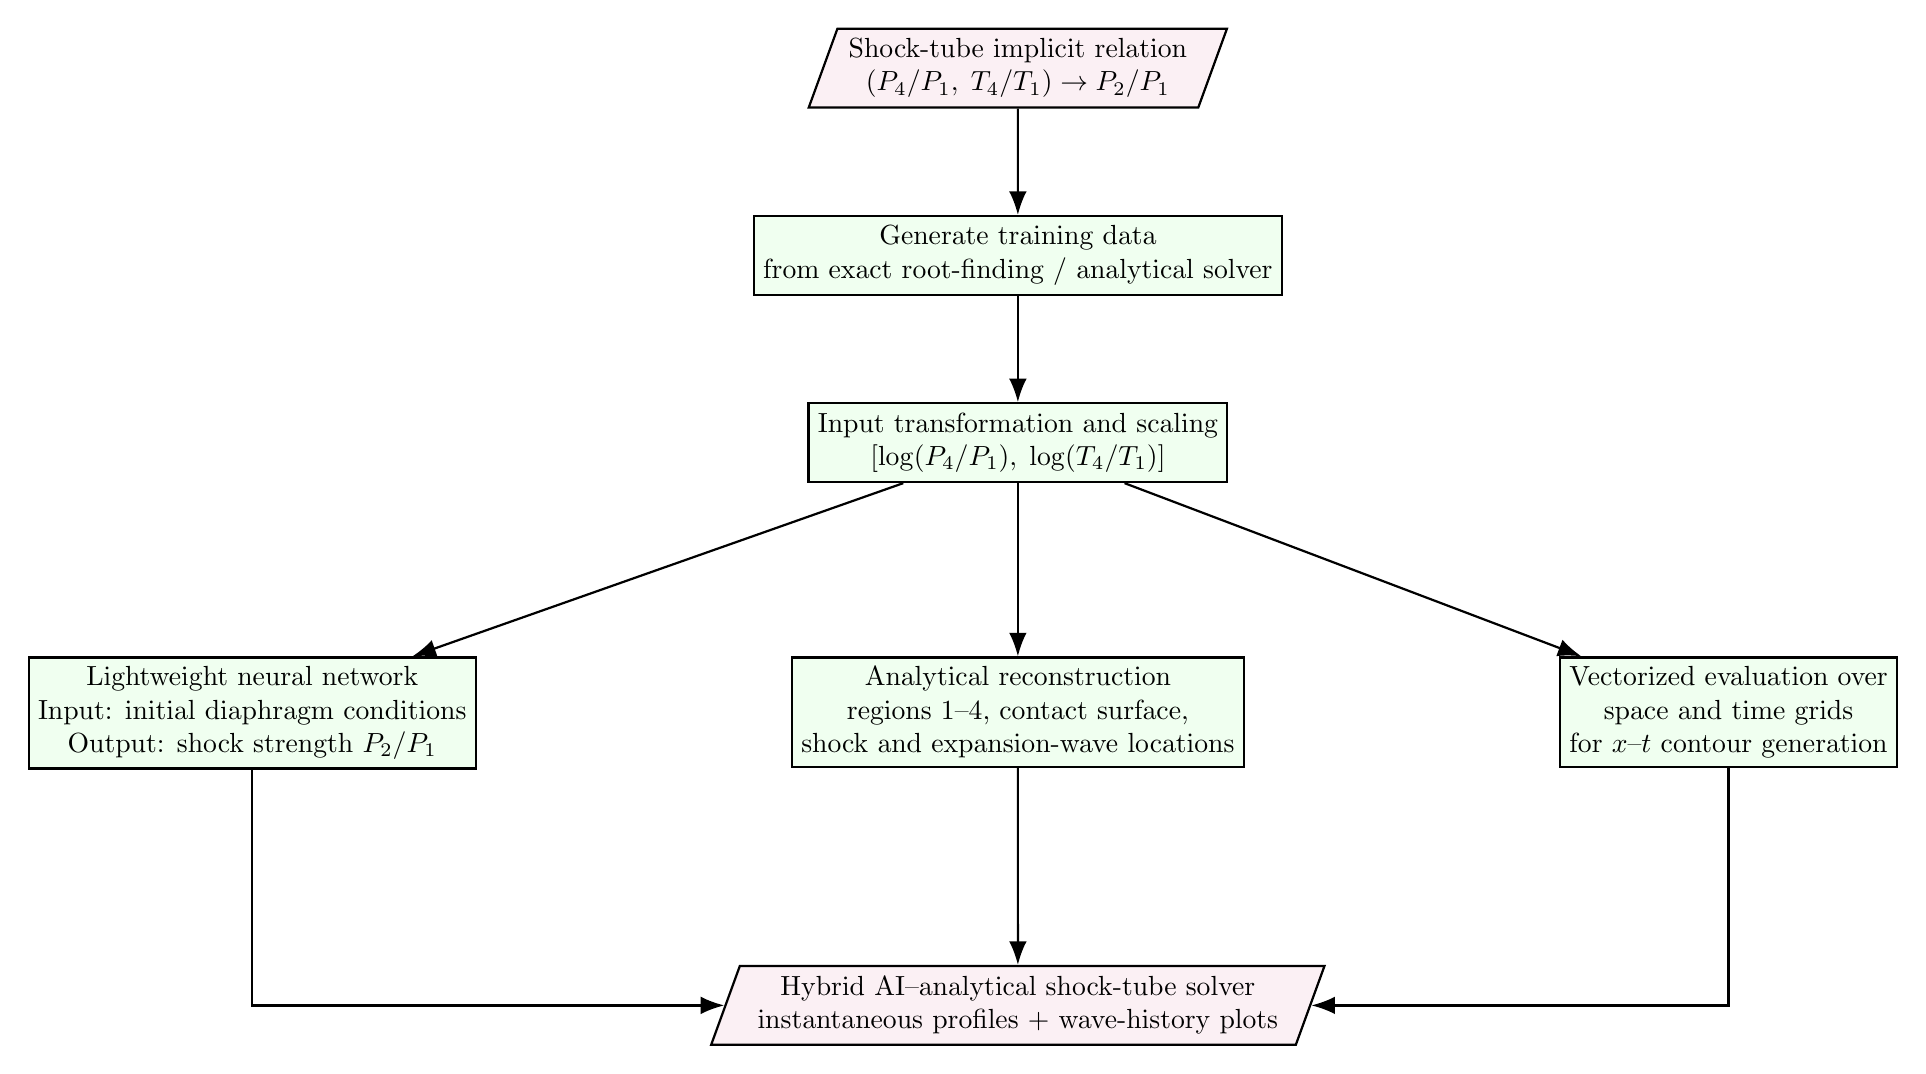
\begin{tikzpicture}[node distance=1.35cm and 1.8cm]

% Top chain
\node[io] (eq) {Shock-tube implicit relation\\ $(P_4/P_1,\;T_4/T_1)\rightarrow P_2/P_1$};

\node[process, below=of eq] (data) {Generate training data\\ from exact root-finding / analytical solver};

\node[process, below=of data] (prep) {Input transformation and scaling\\ $[\log(P_4/P_1),\;\log(T_4/T_1)]$};

% Middle row
\node[process, below left=2.2cm and 4.2cm of prep] (train) {Lightweight neural network\\ Input: initial diaphragm conditions\\ Output: shock strength $P_2/P_1$};

\node[process, below=2.2cm of prep] (recon) {Analytical reconstruction\\ regions 1--4, contact surface,\\ shock and expansion-wave locations};

\node[process, below right=2.2cm and 4.2cm of prep] (xt) {Vectorized evaluation over\\ space and time grids\\ for $x$--$t$ contour generation};

% Bottom output
\node[io, below=2.5cm of recon] (out) {Hybrid AI--analytical shock-tube solver\\ instantaneous profiles + wave-history plots};

% Arrows
\draw[line] (eq) -- (data);
\draw[line] (data) -- (prep);

\draw[line] (prep) -- (train);
\draw[line] (prep) -- (recon);
\draw[line] (prep) -- (xt);

\draw[line] (train) |- (out);
\draw[line] (recon) -- (out);
\draw[line] (xt) |- (out);

\end{tikzpicture}%
}
\captionof{figure}{Hybrid AI--analytical workflow for the shock-tube surrogate. Training data are generated from the exact implicit shock-tube relation. The neural network is trained only to predict the shock strength from the initial diaphragm state, while the remaining thermodynamic states and wave trajectories are reconstructed analytically. This hybrid design enables both instantaneous flow-profile prediction and rapid generation of space--time wave diagrams.}
\label{fig:shocktube_flowchart}
\end{center}
\end{landscape}
\end{document}
